\section{Pianificazione}
\label{pianificazione}
Considerate le scadenze scelte in sottosezione \S\ref{sub:scadenze_fissate} ed il modello di sviluppo scelto presente nella sezione \S\ref{modello_di_sviluppo}, {\Gruppo} ha suddiviso il progetto in 5 periodi:
\begin{itemize}
    \item \textbf{Analisi};
    \item \textbf{Consolidamento requisiti};
    \item \textbf{Progettazione architetturale};
    \item \textbf{Progettazione di dettaglio e codifica};
    \item \textbf{Validazione e collaudo}.
\end{itemize}
Ogni periodo è caratterizzato da precondizioni, postcondizioni ed è diviso in diversi \glo{stadi temporali}. Ognuno di questi cinque periodi sarà formato da \glo{attività} mostrate nei corrispettivi \glo{diagrammi di Gantt}.Ogni attività si ramifica in sotto-attività per mostrarne l'esecuzione ad alto livello.

\subsection{Analisi}
\label{analisi}
\textbf{Durata:} dal 2020\_11\_06 al 2021\_01\_11\\
Durante questo periodo si forma il gruppo che si prepara alla \glo{\textbf{RR}}, studiando i \glo{capitolati} proposti e svolgendo un'analisi preliminare dei requisiti e la pianificazione globale del lavoro da svolgere. 
Le precondizioni sono:
\begin{itemize}
    \item Formazione del gruppo;
    \item Presentazione dei \glo{capitolati}.
\end{itemize}
Le postcondizioni sono:
\begin{itemize}
    \item Scelta del nome e del logo del gruppo;
    \item Creazione della mail e di un \glo{repository} \glo{GitHub};
    \item Scelta del capitolato;
    \item Redazione dei documenti quali: {\SdF}, {\NdP}, {\PdP}, {\Glossario}, \textit{Lettera di presentazione}, {\PdQ}, {\AdR} ed i verbali;
    \item Verifica e approvazione di quanto redatto.
\end{itemize}
Questa periodo è composto da sette attività che corrispondono ai documenti prodotti:
\begin{itemize}
    \item \textbf{Studio di fattibilità:} Vengono analizzati i vari capitolati per evidenziarne gli aspetti negativi e positivi. Dopo un periodo di studio e confronto {\Gruppo} dà la preferenza in quello più adatto. L'attività è bloccante per l'{\AdR};
    \item \textbf{Norme di progetto:} Vengono definite tutte le regole che il gruppo {\Gruppo} dovrà seguire per la stesura dei documenti e per lo sviluppo del progetto;
    \item \textbf{Glossario:} Contiene tutti i termini che possono risultare ambigui durante lo svolgimento del progetto; di essi viene fornita una definizione sintetica ed esaustiva;
    \item \textbf{Lettera di presentazione:} Documento in cui il gruppo {\Gruppo} si candida al capitolato scelto come fornitore del prodotto software richiesto;
    \item \textbf{Piano di progetto:} Nel presente documento sono descritte le attività, i rischi del progetto e viene calcolato il preventivo per la realizzazione di progetto. Presenta poi la suddivisione del lavoro tra i membri del gruppo {\Gruppo} e il calcolo del preventivo;
    \item \textbf{Analisi dei requisiti:} Vengono studiati e analizzati nel dettaglio i requisiti del capitolato scelto nello {\SdF};
    \item \textbf{Piano di qualifica:} Si individuano metodi e procedure per garantire la \glo{qualità} del prodotto.
\end{itemize}
La pianificazione di questo periodo è stata organizzata nel modo seguente:
\begin{enumerate}
\item \textbf{2020\_11\_06 - 2020\_12\_03}:
Inizio della stesura delle {\NdP} per avere delle regole condivise dal gruppo per svolgere il lavoro. Durante la stesura di queste, il gruppo si confronta riguardo ai vari capitolati esponendo le preferenze personali di ciascun componente del gruppo. Viene analizzato ogni capitolato focalizzando l'attenzione principalmente verso i loro aspetti positivi e negativi e dei possibili rischi che si possono incontrare per ognuno. Dopo i confronti iniziali si è potuto iniziare uno studio sulla fattibilità generico per tutti i capitolati per poi approfondirlo per i capitolati che suscitavano più interesse al gruppo e iniziare a stilare il {\Glossario} per la registrazione dei termini, usati nei documenti, che potrebbero creare ambiguità. Durante questo periodo sono state prese decisioni tecniche e organizzative come: nome del gruppo, logo, indirizzo mail, creazione \glo{repository} e i vari mezzi di comunicazione. Vengono trascritti i verbali interni relativi alle riunioni del gruppo durante questo arco di tempo;
\item \textbf{2020\_12\_04 - 2020\_12\_21}:
Inizio della stesura del {\PdP}, contenente la pianificazione del lavoro da svolgere e la suddivisione dei ruoli tra i membri del gruppo. Stesa una prima bozza della \textit{Lettera di presentazione}, il cui completamento sarà fatto dopo la conclusione del {\PdP} con l'aggiunta del prospetto economico finale. Integrato il {\Glossario} quando necessario. In data 2020\_12\_22 il gruppo ha fissato una \glo{milestone} per il completamento dei documenti iniziati durante questo periodo, ad eccezione dell'ultima sezione del {\PdP} destinata al consuntivo finale del periodo successivo. Iniziano le attività di verifica incrementale per i documenti in corso di stesura. Stesi i verbali interni relativi agli incontri svolti;
\item \textbf{2020\_12\_22 - 2021\_01\_07}:
Inizio della stesura dell'{\AdR} e del {\PdQ}, con l'esposizione dei criteri di valutazione della qualità scelti dal gruppo e le rispettive metriche di calcolo. Continuano le attività di verifica incrementale per i documenti in corso di stesura;
\item \textbf{2021\_01\_08 - 2021\_01\_11}
Il gruppo svolge le ultime attività di verifica sugli ultimi documenti, completa il {\Glossario} e uniforma tutti i prodotti alle regole stabilite nelle {\NdP} se necessario.
\end{enumerate}
\subsubsection{Diagramma di Gantt: Analisi}
\begin{figure}[ht]
    \centering
    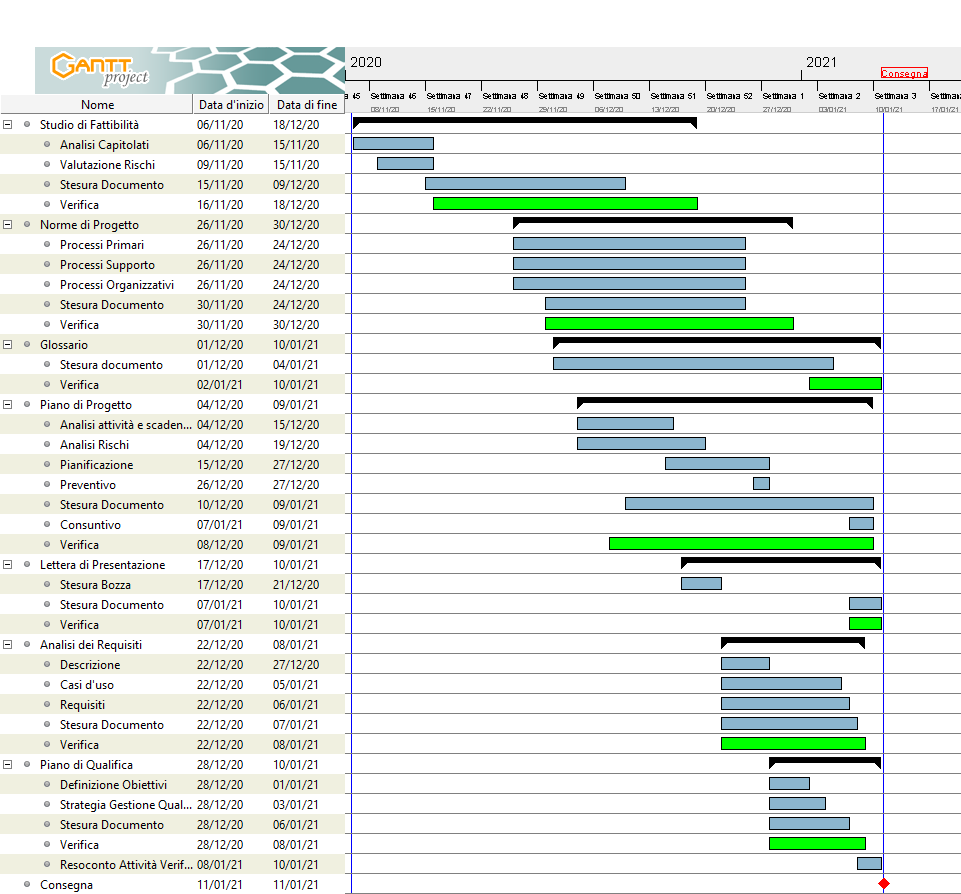
\includegraphics[width=\textwidth]{Immagini/GanttAnalisi}
    \caption{Diagramma di Gantt dell'attività di analisi}
\end{figure}
\newpage
\subsection{Consolidamento Requisiti}
\label{consolidamento_requisiti}
\textbf{Durata:} dal 2020-01-11 al 2020-01-18 \\
In questo periodo il gruppo si prepara alla propria presentazione in vista della \textit{Revisione dei Requisiti}.
I componenti si dividono gli argomenti da esporre e descrivono il lavoro svolto durante l'analisi attraverso delle diapositive.
I membri del team si occupano di approfondire individualmente la propria conoscenza delle tecnologie che verranno utilizzate successivamente.

Le precondizioni sono:
\begin{itemize}
    \item Le postcondizioni del periodo precedente sono state soddisfatte;
    \item Consegna dei documenti richiesti al proponente.
\end{itemize}

Le postcondizioni sono:
\begin{itemize}
    \item Ultimata preparazione della presentazione da esporre in sede di revisione;
    \item Ogni componente ha studiato le tecnologie necessarie;
\end{itemize}
Le attività che vengono svolte sono:
\begin{itemize}
    \item Miglioramento dei documenti e verifica;
    \item Preparazione alla presentazione per la \textit{Revisione dei Requisiti};
    \item Ogni componente dovrà svolgere dello studio autonomo per approfondire le tecnologie necessarie nei periodi successivi.  
\end{itemize}

\newpage
\subsubsection{Diagramma di Gantt: Consolidamento Requisiti}
\begin{figure}[ht]
    \centering
    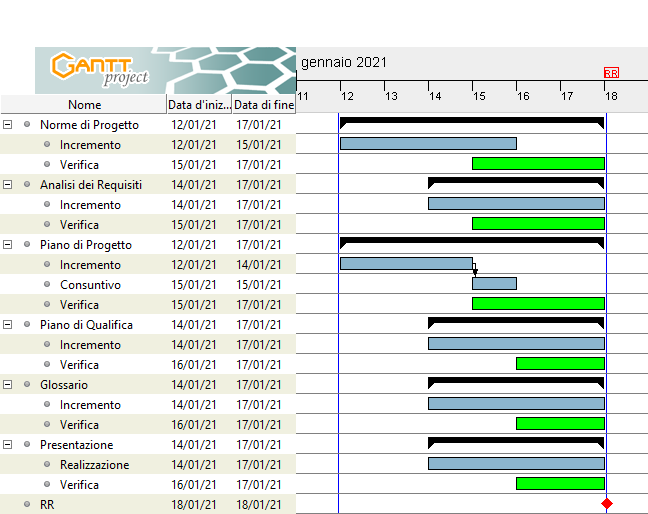
\includegraphics[width=\textwidth]{../../Immagini/GanttConsolidamentoRequisiti}
    \caption{Diagramma di Gantt dell'avvitià di Consolidamento dei Requisiti}
\end{figure}

\newpage
\subsection{Progettazione Architetturale}

\textbf{Periodo:} dal 2020-01-18 al 2020-03-08
\\La fase inizia appena conclusa la precedente e termina con la Revisione di Progettazione.
\\Le precondizioni sono:

\begin{itemize}
    \item Le postcondizioni della fase precedente sono state soddisfatte;
    \item La candidatura del gruppo al progetto \NomeProgetto è stata accolta.
\end{itemize}
    Le postcondizioni sono:
\begin{itemize}
    \item Aggiornamento e correzione dei documenti già prodotti;
    \item Produzione del Proof of Concept;
    \item Completamento della progettazione ad alto livello del software;
    \item Consegna dei documenti richiesti in entrata allaRevisione di Progettazione;
    \item Ultimata preparazione della presentazione da esporre in sede di revisione.
\end{itemize}

\subsubsection{Attività}

\subsubsection{Periodi}

\subsubsection{Diagramma di Gantt: Progettazione Architetturale}

\newpage
\subsection{Progettazione di dettaglio e codifica}
\label{progettazione_di_dettaglio}
\textbf{Durata:} dal 2021\_03\_09 al 2021\_04\_02 \\
Il periodo inizia appena concluso il precedente e termina con la \glo{\textbf{RQ}}.
Le precondizioni sono:
\begin{itemize}
    \item Le postcondizioni del periodo precedente sono state soddisfatte.
\end{itemize}
Le postcondizioni sono:
\begin{itemize}
    \item Aggiornamento e correzione dei documenti già prodotti;
    \item Realizzazione dei diagrammi delle classi e delle attività;
    \item Completamento codifica e relativa verifica;
    \item Redazione \textbf{manuale utente} e \textbf{manuale sviluppatore};
    \item Consegna dei documenti richiesti in entrata alla \textbf{RQ};
    \item Ultimata preparazione della presentazione da esporre in sede di revisione.
\end{itemize}
È composto da nuovi incrementi e nuove attività:
\begin{itemize}
    \item \textbf{Incremento e verifica dei documenti (dal 2021\_03\_09 al 2021\_03\_26):} i documenti già prodotti vengono migliorati e aggiornati se necessario ({\NdP}, {\PdP}, {\Glossario}, {\PdQ}, {\AdR});
    \item \textbf{Incremento e verifica delle attività (dal 2021\_03\_09 al 2021\_03\_17)}: viene migliorata l'attività di \glo{TB}, ampliando lo studio delle tecnologie mancanti e progettando ad alto livello come realizzare il prodotto finale;
    \item \textbf{Product Baseline (dal 2021\_03\_09 al 2021\_03\_17):} segue la Technology Baseline e vengono discussi:
        \begin{itemize}
            \item \textbf{Design pattern}: vengono individuati e discussi in modo da capire quali siano necessari e come riuscire a integrarli al meglio nel progetto;
            \item \textbf{Diagrammi classi}: dopo un'attenta riflessione sul codice vengono realizzati i diagrammi delle classi;
            \item \textbf{Diagrammi attività}: dopo un'attenta riflessione sul codice vengono realizzati i diagrammi delle attività. 
        \end{itemize} 
    \item \textbf{Specifica tecnica(dal 2021\_03\_18 al 2021\_03\_26):} viene realizzato un documento contenente tutte le caratteristiche del prodotto e le motivazioni che hanno portato alla loro scelta;
    \item \textbf{Codifica (dal 2021\_03\_18 al 2021\_04\_06):} viene scritto il codice con relativa verifica. Questa attività, dato il modello di sviluppo scelto, verrà suddivisa in 3 incrementi che verranno definiti dopo aver preparato il Proof of Concept così da avere una maggiore conoscenza sul lavoro effettivo da svolgere e poter progettare al meglio i vari incrementi;
    \item \textbf{Manuale utente e manutentore(dal 2021\_03\_24 al 2021\_04\_06):} documenti redatti rispettivamente per indicare le istruzioni d'uso specifiche per l'utente e per supportare eventuali sviluppatori attraverso la descrizione dell'architettura del sistema.
\end{itemize}
\subsubsection{Incrementi del periodo}\label{IncrementiPDettaglio}
\begin{table}[H]
	\begin{center}
		\begin{tabular}{ |C{3cm} C{6cm} C{7cm}| }
			\rowcolor{darkblue} 
			\textcolor{white}{\textbf{Incremento}} & \textcolor{white}{\textbf{Obiettivi}} & \textcolor{white}{\textbf{Requisiti}} \\ \hline
			I dal 2021\_03\_09 al 2021\_03\_17& Miglioramento della documentazione già prodotta, ampliamento dello studio delle tecnologie, studio di \glo{design pattern}, diagrammi delle classi e delle attività.  & - \\ \hline
			II dal 2021\_03\_18 al 2021\_03\_26 	& Correzione dei documenti post \glo{RP}, redazione dell'allegato tecnico, inizio sviluppo del codice e redazione manuali. &  
			RFO1\_1 - RFO6\_1.1.5, RFO7\_2 \newline
			RFO8\_3, RFO10\_4, RFO11\_5 \newline
			RFO59, RFO60 \newline
			RFO61\_23 - RFO62\_23.4, RFO67\_25 \newline
			RF069, RFO70\_26 - RFO77\_26.7 \newline
			RFO78, RFO79, RFO12\_6, \newline 
			RFO13\_ 7 - RFO15\_ 7.3, RFO17 \newline RFO18, RFO19, RFO20\_8\newline RFO21\_9, RFO22\_10, RFO23\_11 \newline RFO24, RFO27, RFO28 \newline RFO29\_12, RFO68, RFO80 \newline RFO81, RFO82, RFO80 \\ \hline
			III dal 2021\_03\_27 al 2021\_04\_01 	& Continuazione nello sviluppo del codice e nella redazione manuali. & RFO81\_27 - RFO88\_27.7 \newline
			RFO89, RFO90\_28 - RFO97\_28.7 \newline
			RFO98\_29, RFO99\_30, RFO100\_31 \newline
			RFO101\_32, RFO102\_33 \newline
			RFO103\_34 - RFO107\_34.4, RFO108 \newline
			RFO109\_35 - RFO110\_35.1\newline
			RFO111\_36 - RFO112\_36.1, RFO113\_37 \newline RFO114\_38, RFO115, RFO26 \newline RFO30\_13, RFO31, RFO32\_14 \newline RFO33\_14, RFO34\_15, RFO35\_16\newline  RFO36, RFO37, RFO41\_17.2 \\ \hline
			III dal 2021\_04\_01 al 2021\_04\_06 	& 
			Conclusione della redazione del codice e dei manuali. & RFO24, RFO41\_17, RFO39\_17.1\newline RFO40,
			RFO41\_17 - RFO45\_17.1.4\newline
			RFO46\_18 - RFO50\_18.4, RFO51\_19 \newline
			RFO52, RFO53\_20, RFO54\_20 \newline
			RFO55\_21, RFO56\_22 - RFO58\_22.2 \newline
			RFO79, RFO116\_39, RFO117\_39 \newline RFO118\_40, RFO119, RFO120\_41 \newline
			RFO121\_42, RFO122\_43 - RFO126\_43.2.2 \\ \hline
		\end{tabular}
		\caption{Tracciamento incrementi-obiettivi}
	\end{center}
\end{table}

\newpage
\subsubsection{Diagramma di Gantt: Progettazione di dettaglio e codifica} \label{GanttPDettaglio}
\begin{figure}[ht]
    \centering
    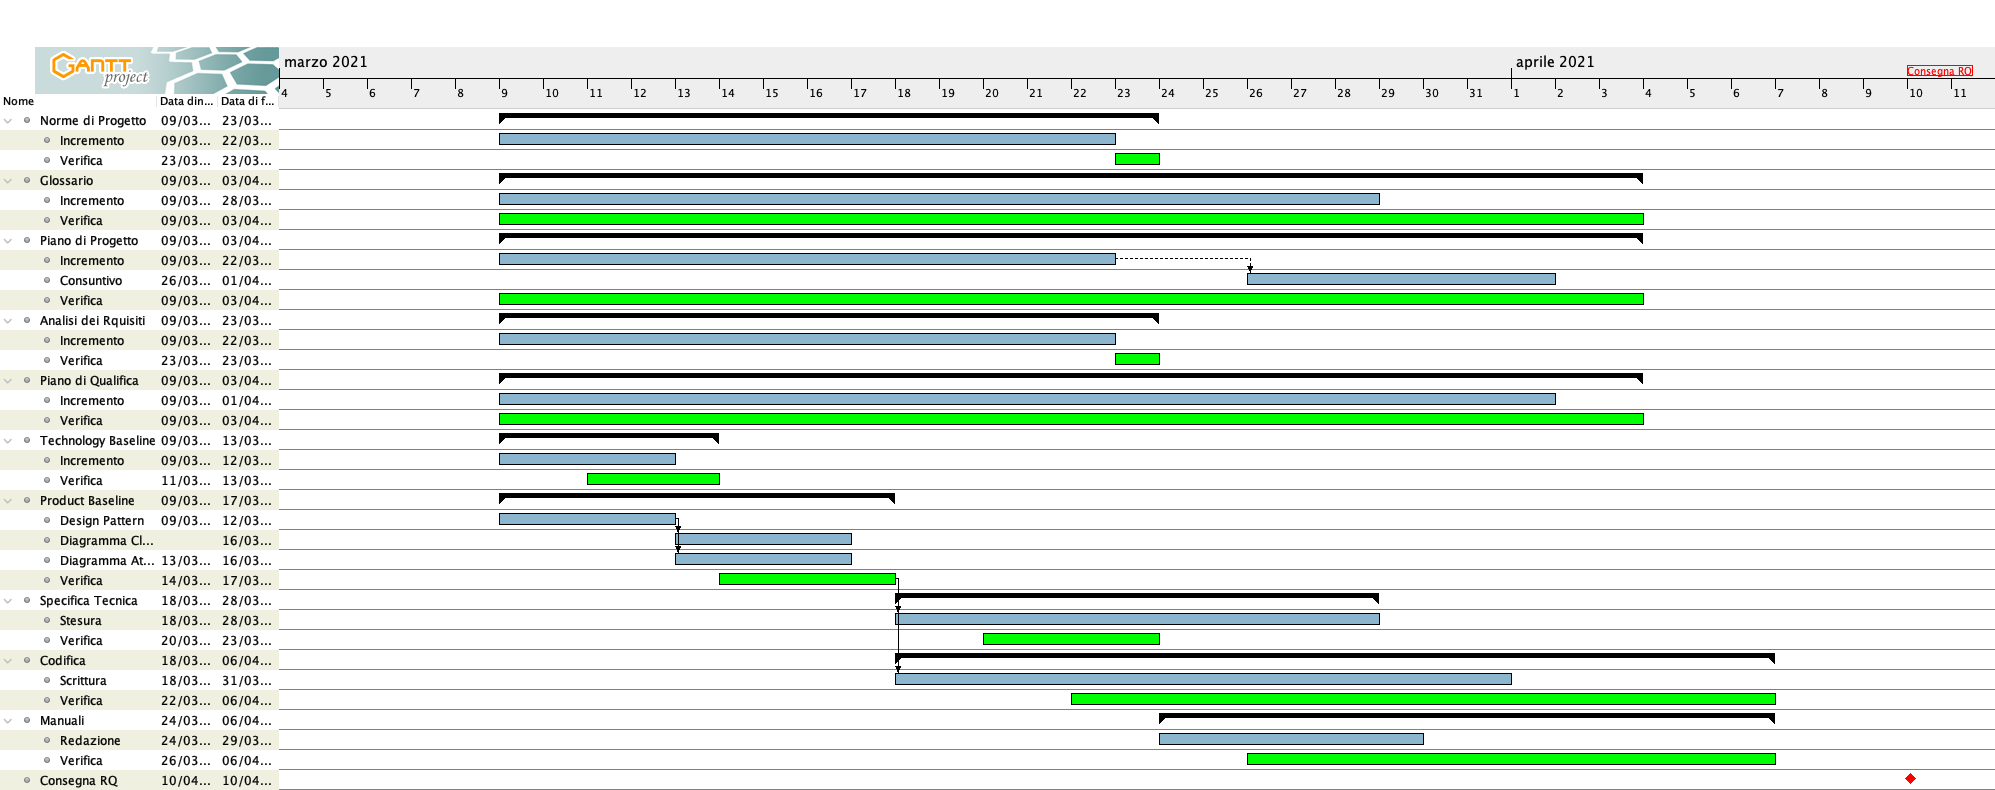
\includegraphics[width=\textwidth]{Immagini/GanttProgettazioneDiDettaglioECodifica}
    \caption{Diagramma di Gantt dell'attività di progettazione di dettaglio e codifica}
\end{figure}
\newpage
\subsection{Validazione e collaudo}
\label{validazione_e_collaudo}
\textbf{Durata:} dal 2021\_05\_01 al 2021\_05\_19\\
Il periodo di validazione e collaudo inizia appena concluso il precedente e termina con la \glo{\textbf{RA}}.
Le precondizioni sono:
\begin{itemize}
    \item Le postcondizioni del periodo precedente sono state soddisfatte.
\end{itemize}
Le postcondizioni sono:
\begin{itemize}
    \item Aggiornamento e correzione documenti già prodotti;
    \item Esecuzione dei vari test;
    \item Completamento del prodotto in base a quanto discusso durante la \textbf{RQ};
    \item Consegna dei documenti richiesti in entrata alla \textbf{RA};
    \item Ultimata preparazione della presentazione da esporre in sede di revisione.
\end{itemize}
È composto da nove incrementi e una nuova attività:
\begin{itemize}
    \item \textbf{Incremento e verifica dei documenti}: alcuni dei documenti già prodotti vengono migliorati e aggiornati ({\NdP}, {\PdP}, {\Glossario}, {\PdQ}, \textit{Specifica tecnica}, \textit{Manuale utente}); 
    \item \textbf{Incremento e verifica delle attività}: se necessario vengono migliorate le attività di \textbf{Technology Baseline} per quanto riguarda la progettazione ad alto livello, in particolare la \textbf{Product Baseline} riguardo all'aggiunta di design pattern o di diagrammi di classi o di attività; la parte di codifica, in caso non siano stati riscontrati rallentamenti o ritardi nel progetto, potrebbe comprendere l'implementazione di uno o più casi d'uso opzionali;
    \item \textbf{Validazione e collaudo}: realizzazione degli ultimi test, con successivi controlli finali per garantire un buon livello di qualità e correttezza.
\end{itemize}
\newpage
\subsubsection{Ripianificazione attuata relativa al periodo} \label{RipianificazioneValidazione}
A seguito dei ritardi accumulati nei periodi precedenti si prevede di consegnare il prodotto verso metà maggio rispettando comunque il preventivo concordato precedentemente e il livello di qualità che il gruppo intende assicurare. Di seguito si riporta il nuovo diagramma di Gantt considerando la nuova data di consegna del prodotto.
\subsubsection{Diagramma di Gantt: Validazione e collaudo}\label{GanttValidazione}
\begin{figure}[ht]
    \centering
    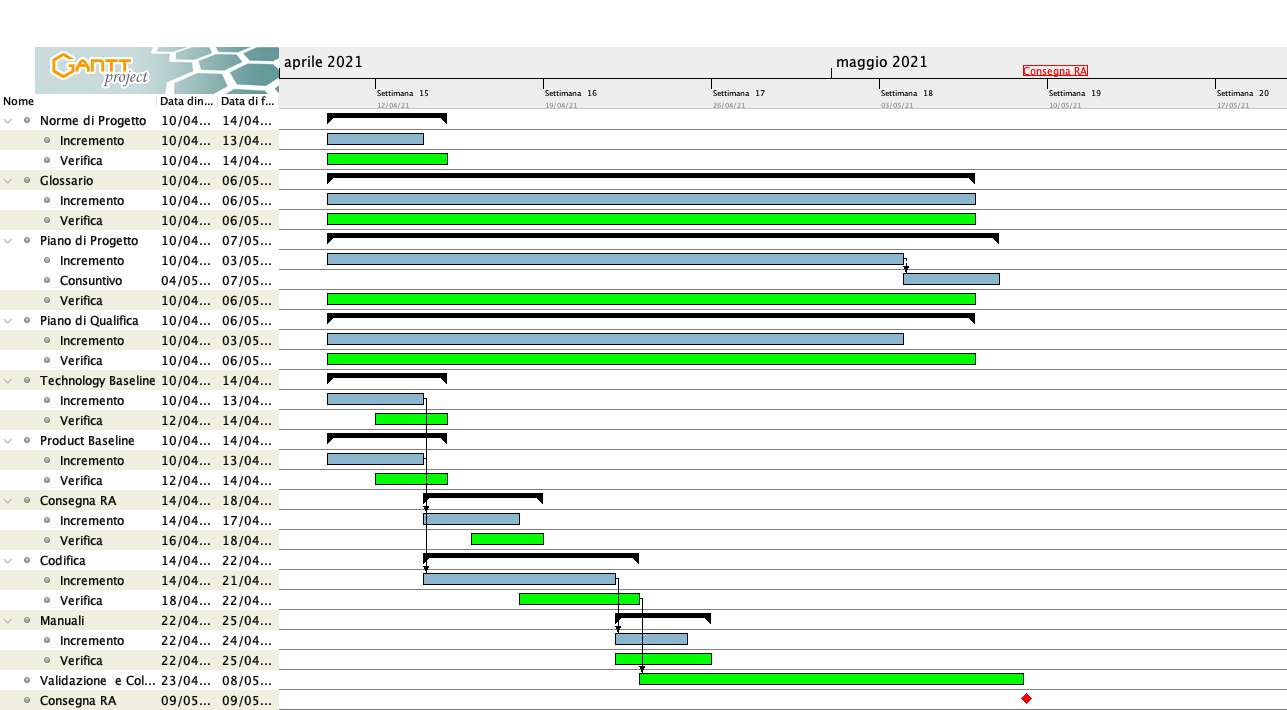
\includegraphics[width=\textwidth]{Immagini/GanttValidazioneECollaudo}
    \caption{Diagramma di Gantt dell'attività di validazione e collaudo}
\end{figure}
\newpage
